\chapter{Análise Estatística do Uso do Sistema de Recomendação}\label{ape:analise-estatistica-do-uso}

\textbf{Links Acessados por Aluno}

\begin{figure}[htb]
  \caption{\label{fig:uso-sr-boxplot}Boxplot dos links acessados por aluno}
  \begin{center}
      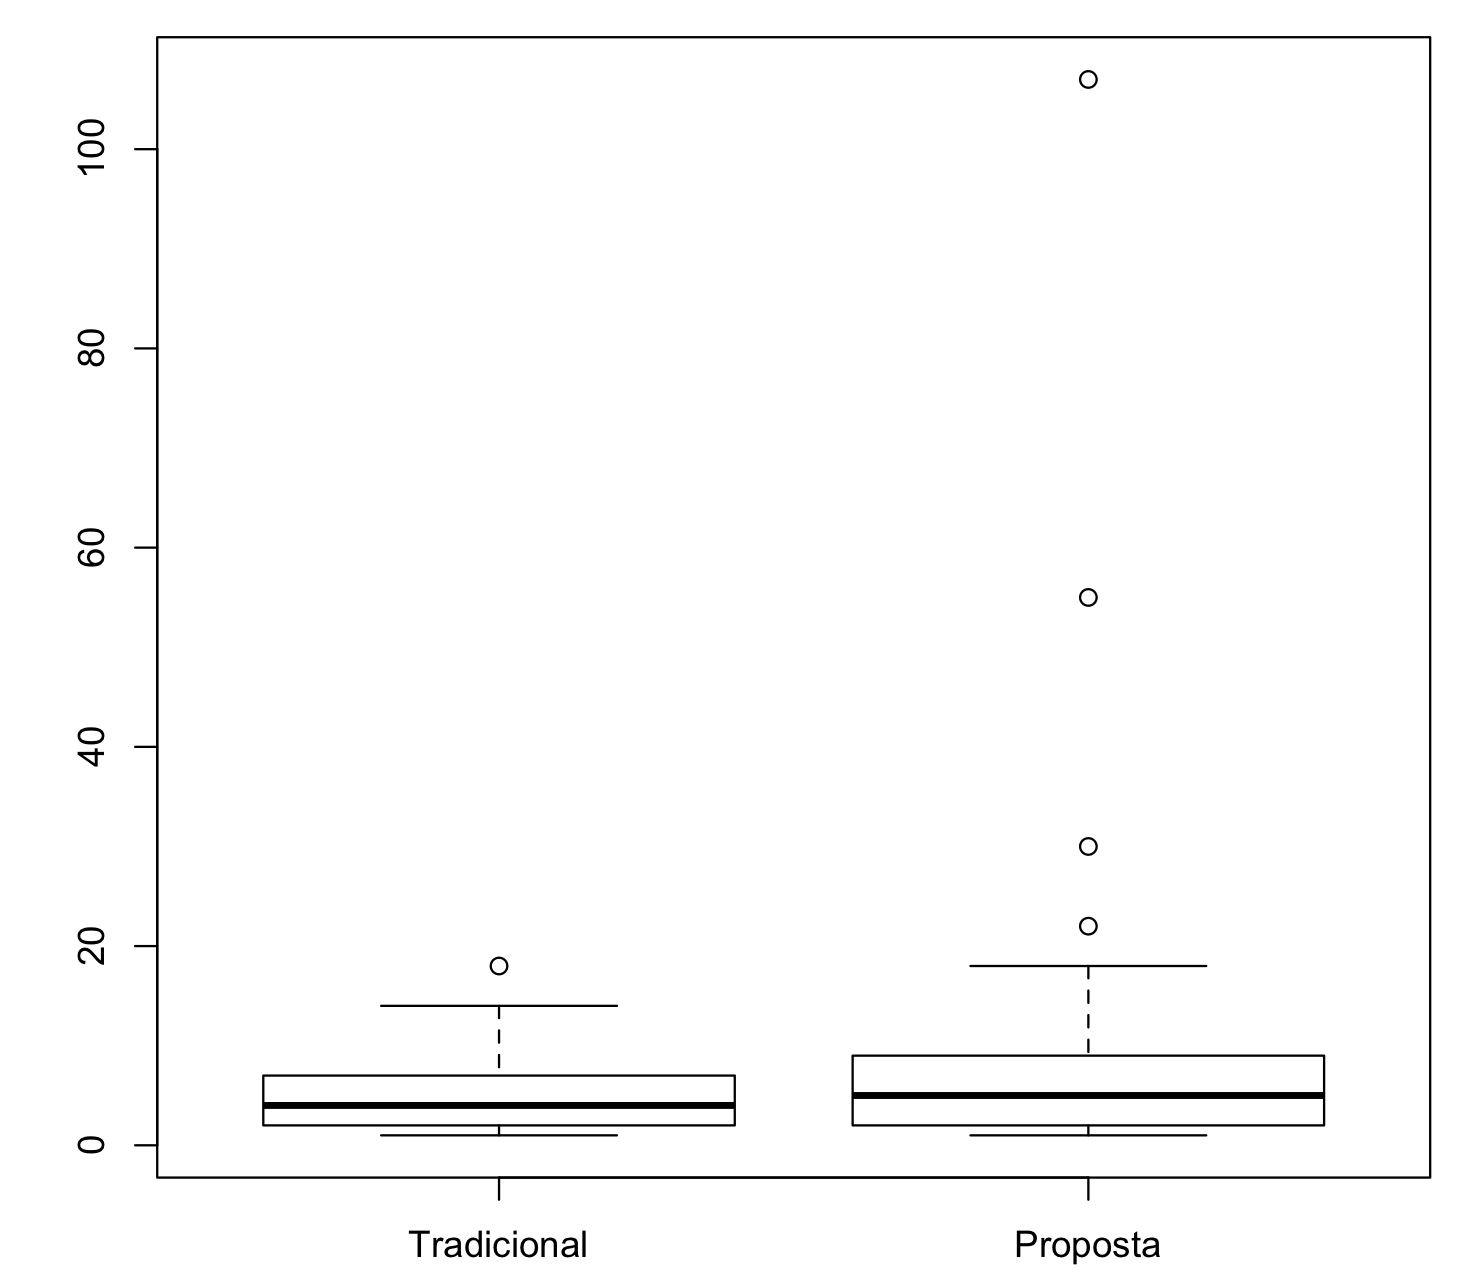
\includegraphics[scale=0.4]{./Figuras/uso-sr-boxplot.png}
  \end{center}
  \legend{Fonte: O autor.}
\end{figure}

Total de alunos comparados: 85

\begin{multicols}{2}

\noindent\textbf{Tradicional}\\
Min.   : 1.000\\
1st Qu.: 2.000\\
Median : 4.000\\
Mean   : 4.935\\
3rd Qu.: 6.500\\
Max.   :18.000\\

\columnbreak

\noindent\textbf{Proposta}\\
 Min.   :  1.00\\
 1st Qu.:  2.00\\
 Median :  5.00\\
 Mean   : 10.15\\
 3rd Qu.:  9.00\\
 Max.   :107.00
\end{multicols}

Shapiro-Wilk normality test

\noindent
data:  data[["quantidade"]]\\
W = 0.42461, p-value < 2.2e-16

\textbf{Resultado: Aceita a hipótese alternativa - Distribuição não normal}

Wilcoxon rank sum test with continuity correction

\noindent
data:  data[["quantidade"]] by data[["algoritmo\_recomendacao"]]\\
W = 820, p-value = 0.4957\\
alternative hypothesis: true location shift is not equal to 0

\textbf{Resultado: Aceita a hipótese nula - Sem diferença significativa}

\textbf{Links Avaliados Positivamente por Aluno}

\begin{figure}[htb]
  \caption{\label{fig:avaliados-positivamente-boxplot}Boxplot dos links avaliados positivamente por aluno}
  \begin{center}
      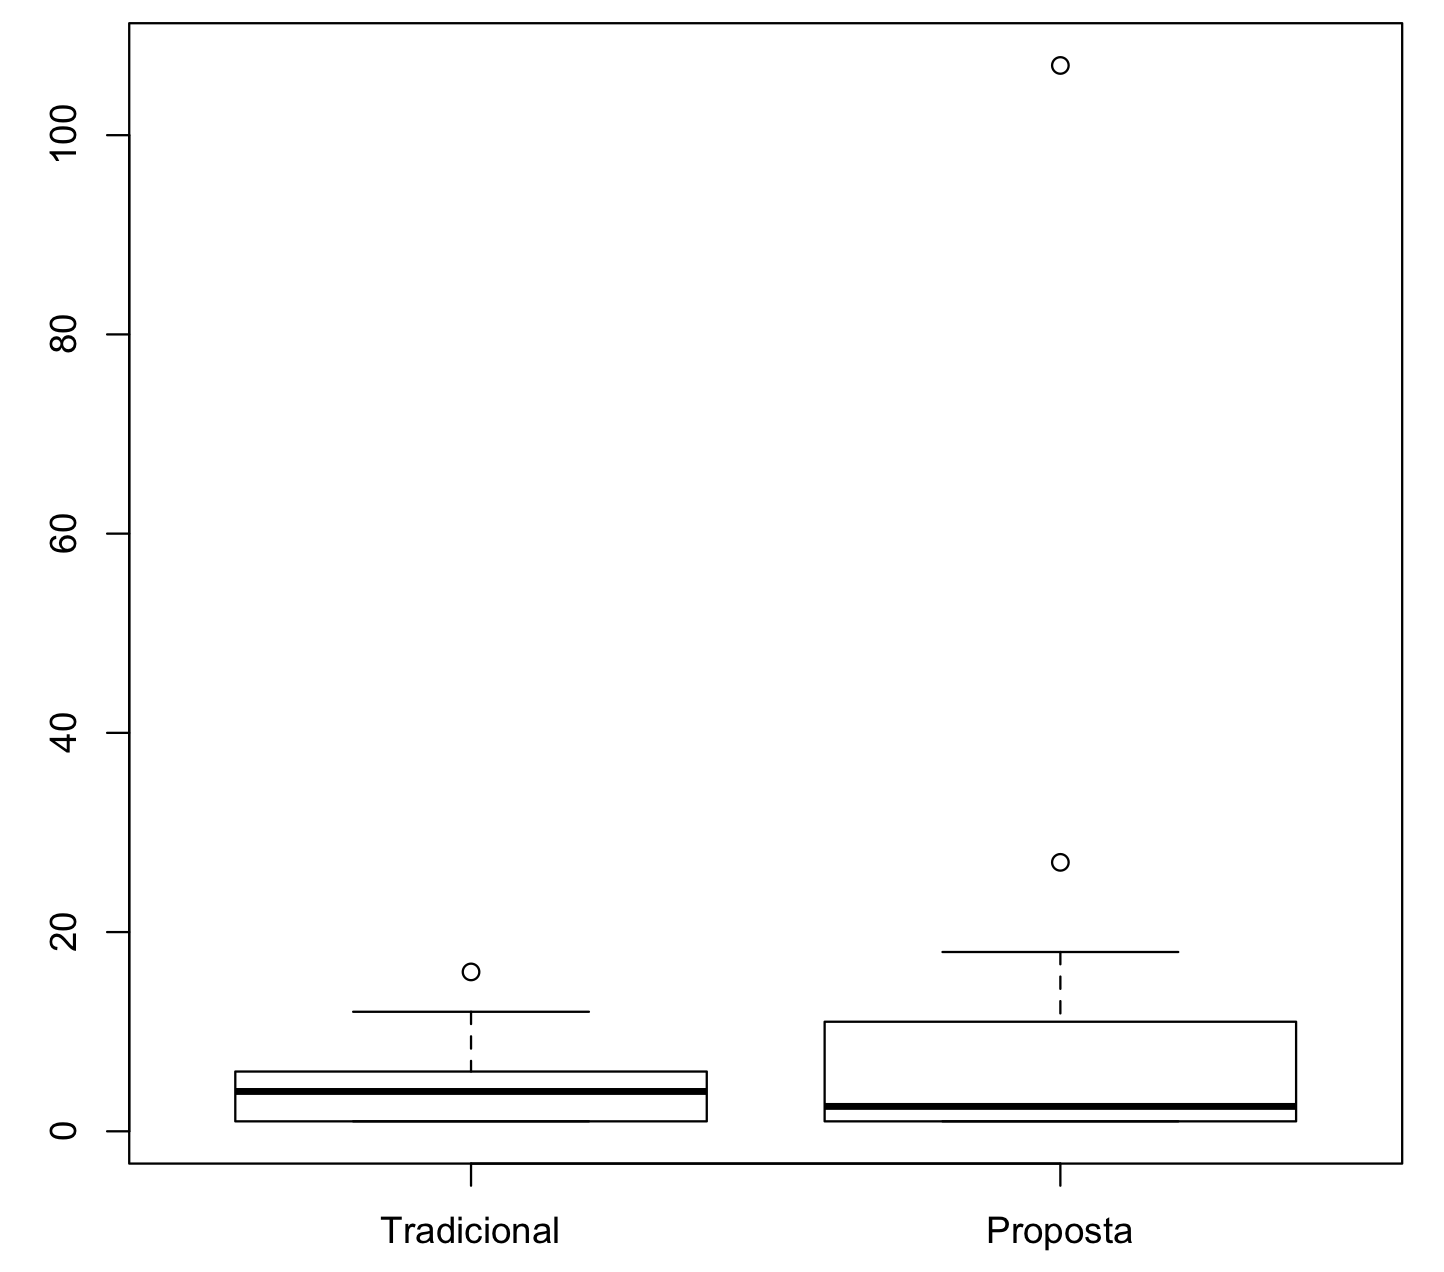
\includegraphics[scale=0.4]{./Figuras/avaliados-positivamente-boxplot.png}
  \end{center}
  \legend{Fonte: O autor.}
\end{figure}

Total de alunos comparados: 52

\begin{multicols}{2}

\noindent\textbf{Tradicional}\\
Min.   : 1.0\\
1st Qu.: 1.0\\
Median : 4.0\\
Mean   : 4.7\\
3rd Qu.: 6.0\\
Max.   :16.0\\

\columnbreak

\noindent\textbf{Proposta}\\
Min.   :  1.00\\
1st Qu.:  1.00\\
Median :  2.50\\
Mean   : 10.64\\
3rd Qu.:  9.75\\
Max.   :107.00
\end{multicols}

  Shapiro-Wilk normality test

\noindent
data:  data[["quantidade"]]\\
W = 0.37836, p-value = 1.654e-13

\textbf{Resultado: Aceita a hipótese alternativa - Distribuição não normal}

Wilcoxon rank sum test with continuity correction

\noindent
data:  data[["quantidade"]] by data[["algoritmo\_recomendacao"]]\\
W = 318, p-value = 0.8275\\
alternative hypothesis: true location shift is not equal to 0

\textbf{Resultado: Aceita a hipótese nula - Sem diferença significativa}

\textbf{Links avaliados negativamente por aluno que acessou pelo menos uma recomendação}

\begin{figure}[htb]
  \caption{\label{fig:uso-sr-boxplot}Boxplot dos links acessados por aluno}
  \begin{center}
      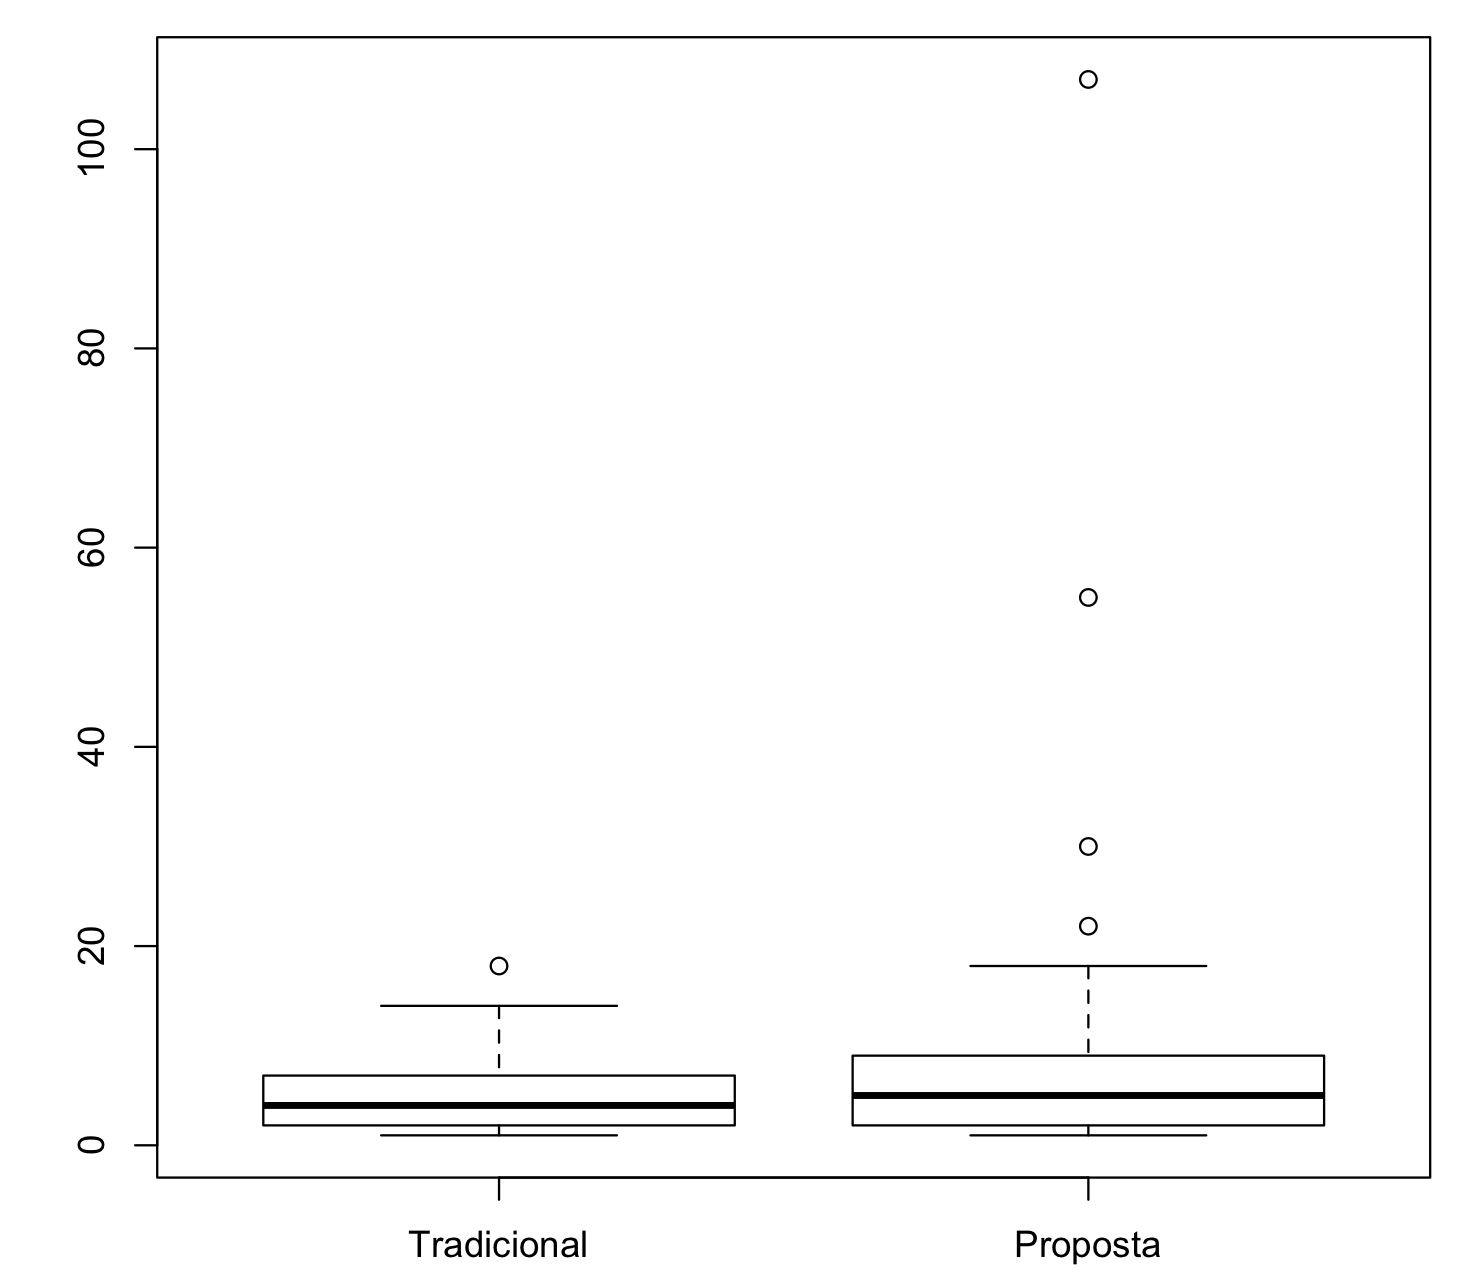
\includegraphics[scale=0.4]{./Figuras/uso-sr-boxplot.png}
  \end{center}
  \legend{Fonte: O autor.}
\end{figure}

Total de alunos comparados: 7

\begin{multicols}{2}

\noindent\textbf{Tradicional}\\
Min.   :1\\
1st Qu.:1\\
Median :1\\
Mean   :1\\
3rd Qu.:1\\
Max.   :1\\

\columnbreak

\noindent\textbf{Proposta}\\
Min.   :1.0\\
1st Qu.:1.5\\
Median :2.0\\
Mean   :2.0\\
3rd Qu.:2.5\\
Max.   :3.0
\end{multicols}

  Shapiro-Wilk normality test

\noindent
data:  data[["quantidade"]]\\
W = 0.45297, p-value = 4.136e-06

\textbf{Resultado: Aceita a hipótese alternativa - Distribuição não normal}

Wilcoxon rank sum test with continuity correction

\noindent
data:  data[["quantidade"]] by data[["algoritmo\_recomendacao"]]\\
W = 2.5, p-value = 0.2059\\
alternative hypothesis: true location shift is not equal to 0

\textbf{Resultado: Aceita a hipótese nula - Sem diferença significativa}

\textbf{Precisão dos algoritmos de recomendação por aluno}

\begin{figure}[htb]
  \caption{\label{fig:precisao-boxplot}Boxplot da precisão dos algoritmos de recomendação por aluno}
  \begin{center}
      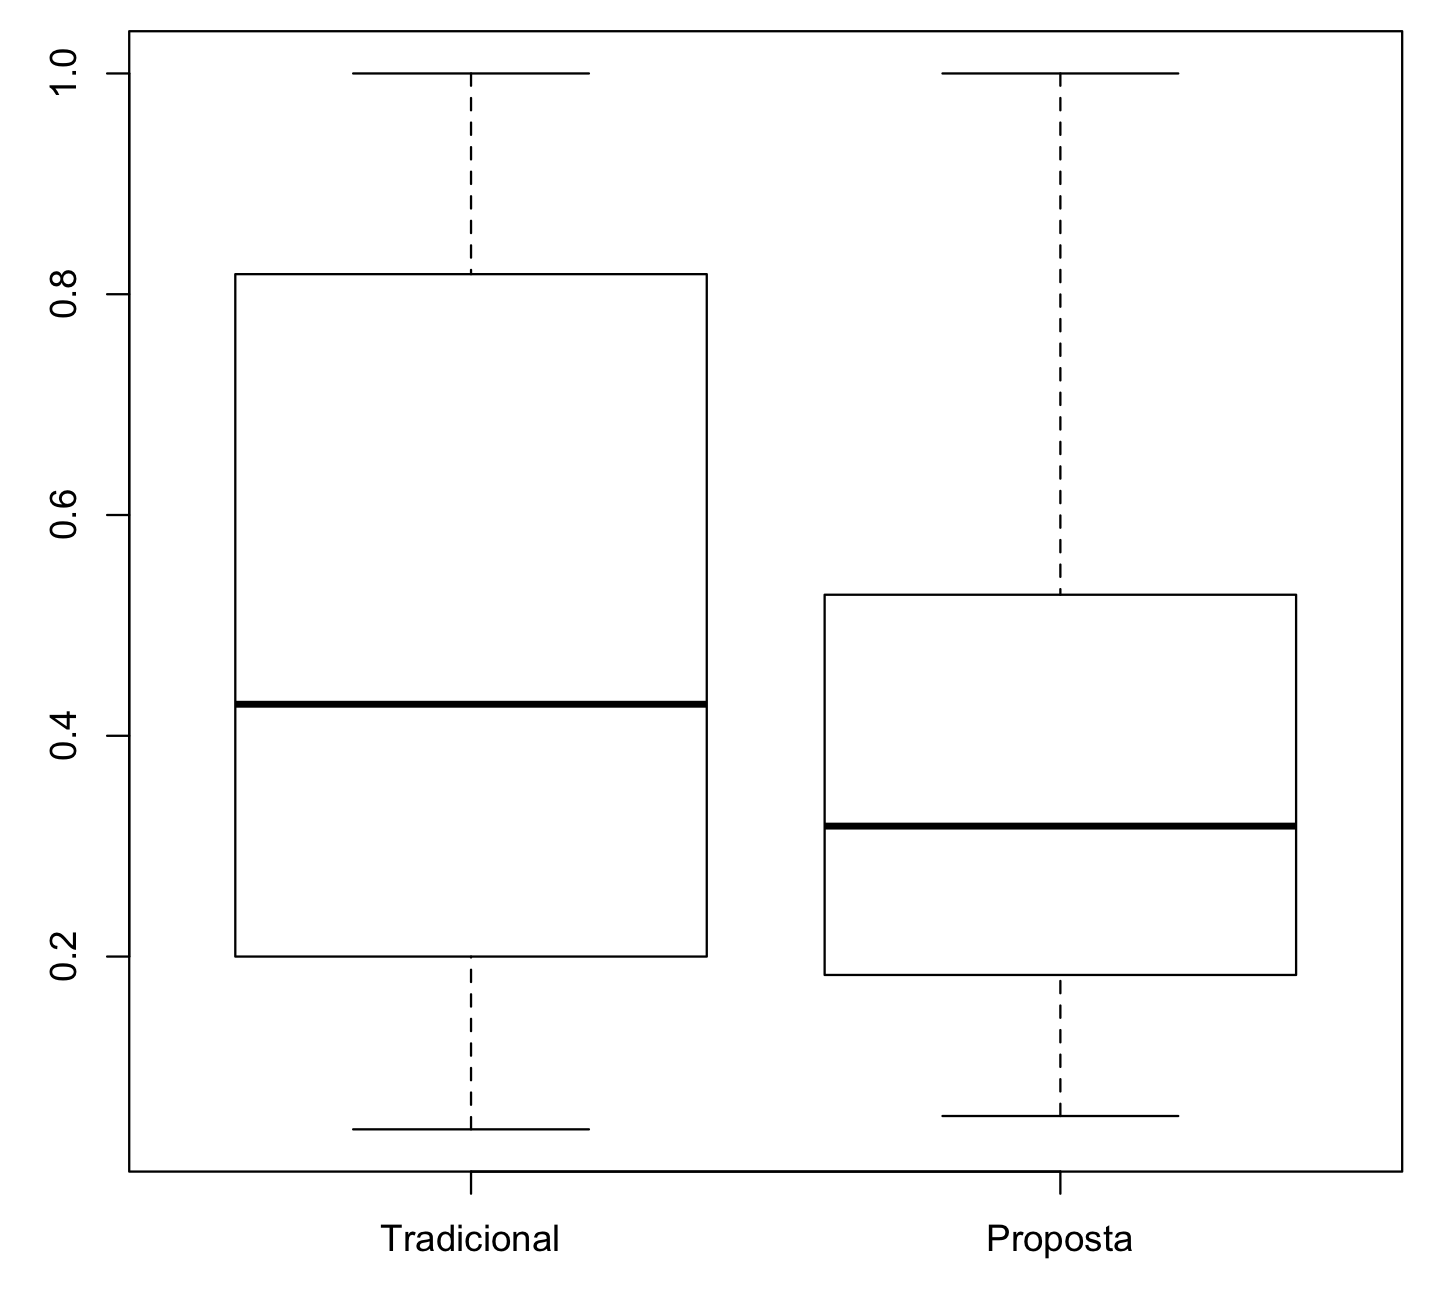
\includegraphics[scale=0.4]{./Figuras/precisao-boxplot.png}
  \end{center}
  \legend{Fonte: O autor.}
\end{figure}

Total de alunos comparados: 85

\begin{multicols}{2}

\noindent\textbf{Tradicional}\\
Min.   :0.04348\\
1st Qu.:0.20000\\
Median :0.42857\\
Mean   :0.49679\\
3rd Qu.:0.81364\\
Max.   :1.00000\\

\columnbreak

\noindent\textbf{Proposta}\\
Min.   :0.05556\\
1st Qu.:0.18333\\
Median :0.31818\\
Mean   :0.39859\\
3rd Qu.:0.52778\\
Max.   :1.00000
\end{multicols}

  Shapiro-Wilk normality test

\noindent
data:  data[["precisao"]]\\
W = 0.89495, p-value = 4.234e-06

\textbf{Resultado: Aceita a hipótese alternativa - Distribuição não normal}

Wilcoxon rank sum test with continuity correction

\noindent
data:  data[["precisao"]] by data[["algoritmo\_recomendacao"]]\\
W = 1025, p-value = 0.2603\\
alternative hypothesis: true location shift is not equal to 0

\textbf{Resultado: Aceita a hipótese nula - Sem diferença significativa}

\textbf{Cobertura dos algoritmos de recomendação por aluno}

\begin{figure}[htb]
  \caption{\label{fig:coverage-boxplot}Boxplot da cobertura dos algoritmos de recomendação por aluno}
  \begin{center}
      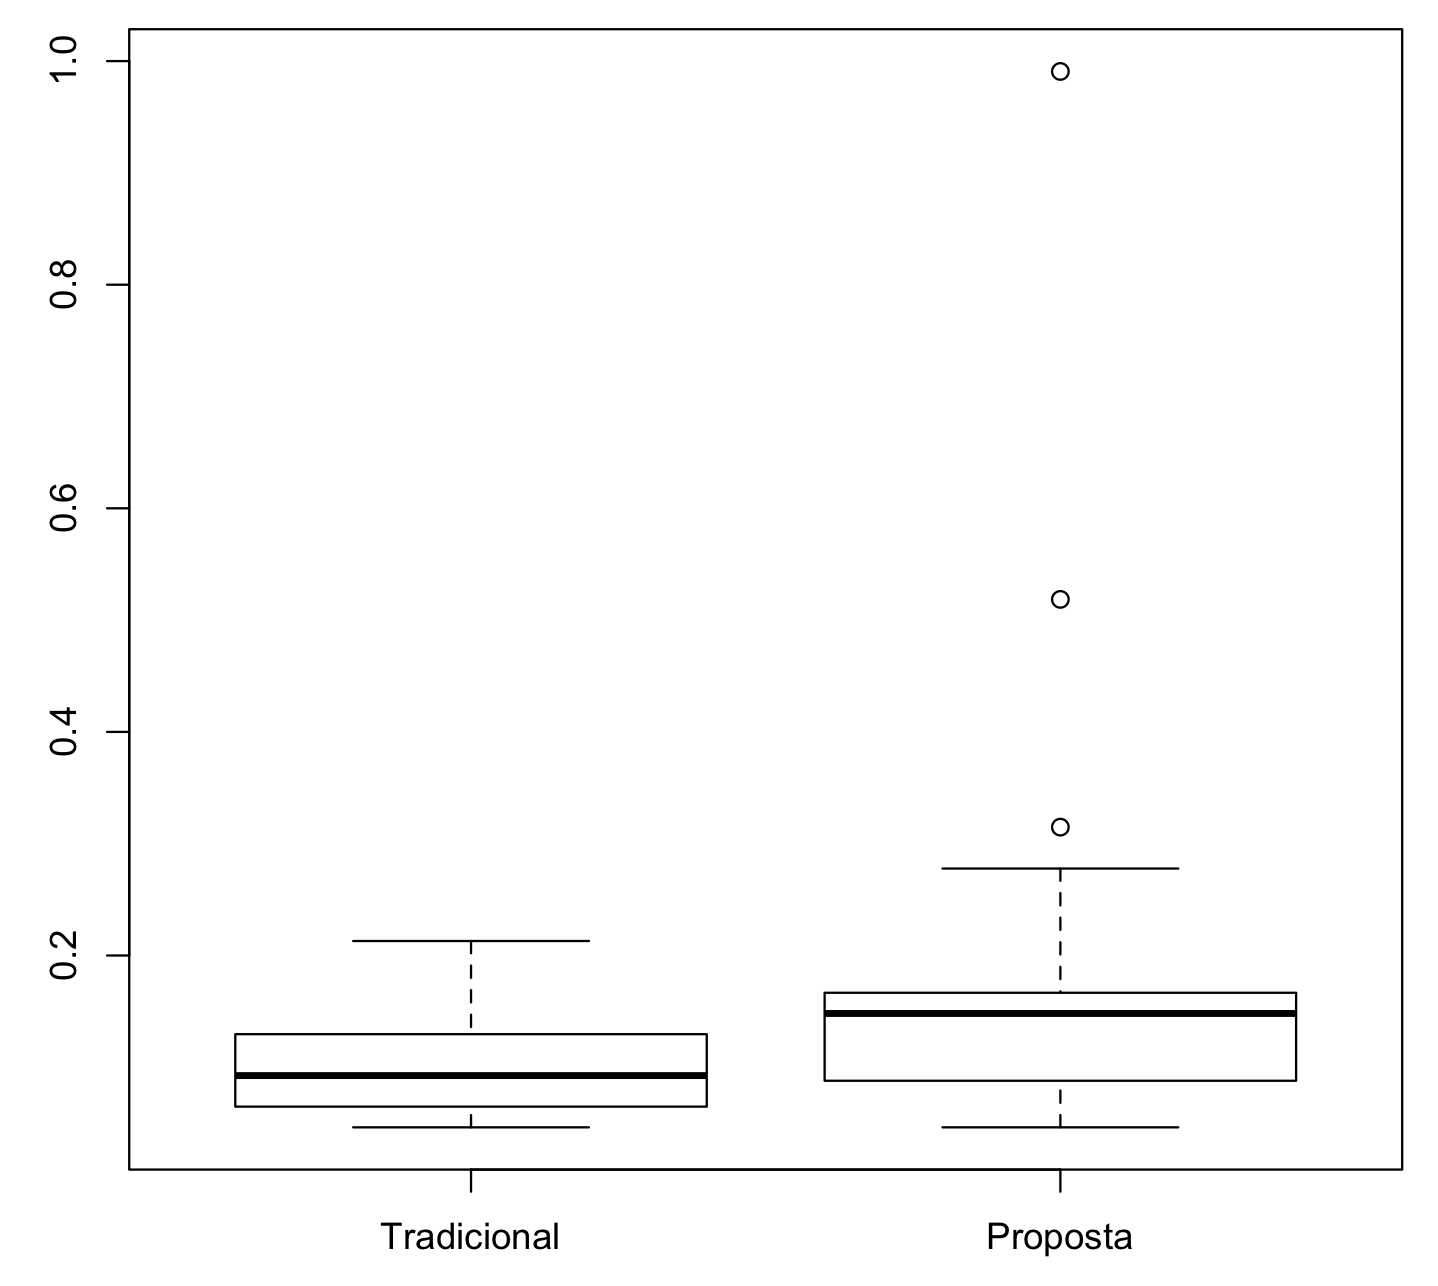
\includegraphics[scale=0.4]{./Figuras/coverage-boxplot.png}
  \end{center}
  \legend{Fonte: O autor.}
\end{figure}

Total de alunos comparados: 85

\begin{multicols}{2}

\noindent\textbf{Tradicional}\\
Min.   :0.04630\\
1st Qu.:0.06481\\
Median :0.09259\\
Mean   :0.10064\\
3rd Qu.:0.12963\\
Max.   :0.21296\\

\columnbreak

\noindent\textbf{Proposta}\\
Min.   :0.04630\\
1st Qu.:0.08796\\
Median :0.14815\\
Mean   :0.17450\\
3rd Qu.:0.16667\\
Max.   :0.99074
\end{multicols}

    Shapiro-Wilk normality test

\noindent
data:  data[["coverage"]]\\
W = 0.55934, p-value = 1.421e-14

\textbf{Resultado: Aceita a hipótese alternativa - Distribuição não normal}

  Wilcoxon rank sum test with continuity correction

\noindent
data:  data[["coverage"]] by data[["algoritmo\_recomendacao"]]\\
W = 525.5, p-value = 0.001031\\
alternative hypothesis: true location shift is not equal to 0

\textbf{Resultado: Aceita a hipótese alternativa - Com diferença significativa}

\textbf{Média harmônica entre Precisão e Cobertura}

\begin{figure}[htb]
  \caption{\label{fig:media-harmonica-boxplot}Boxplot da Média harmônica entre a Precisão e a Cobertura dos dois algoritmos}
  \begin{center}
      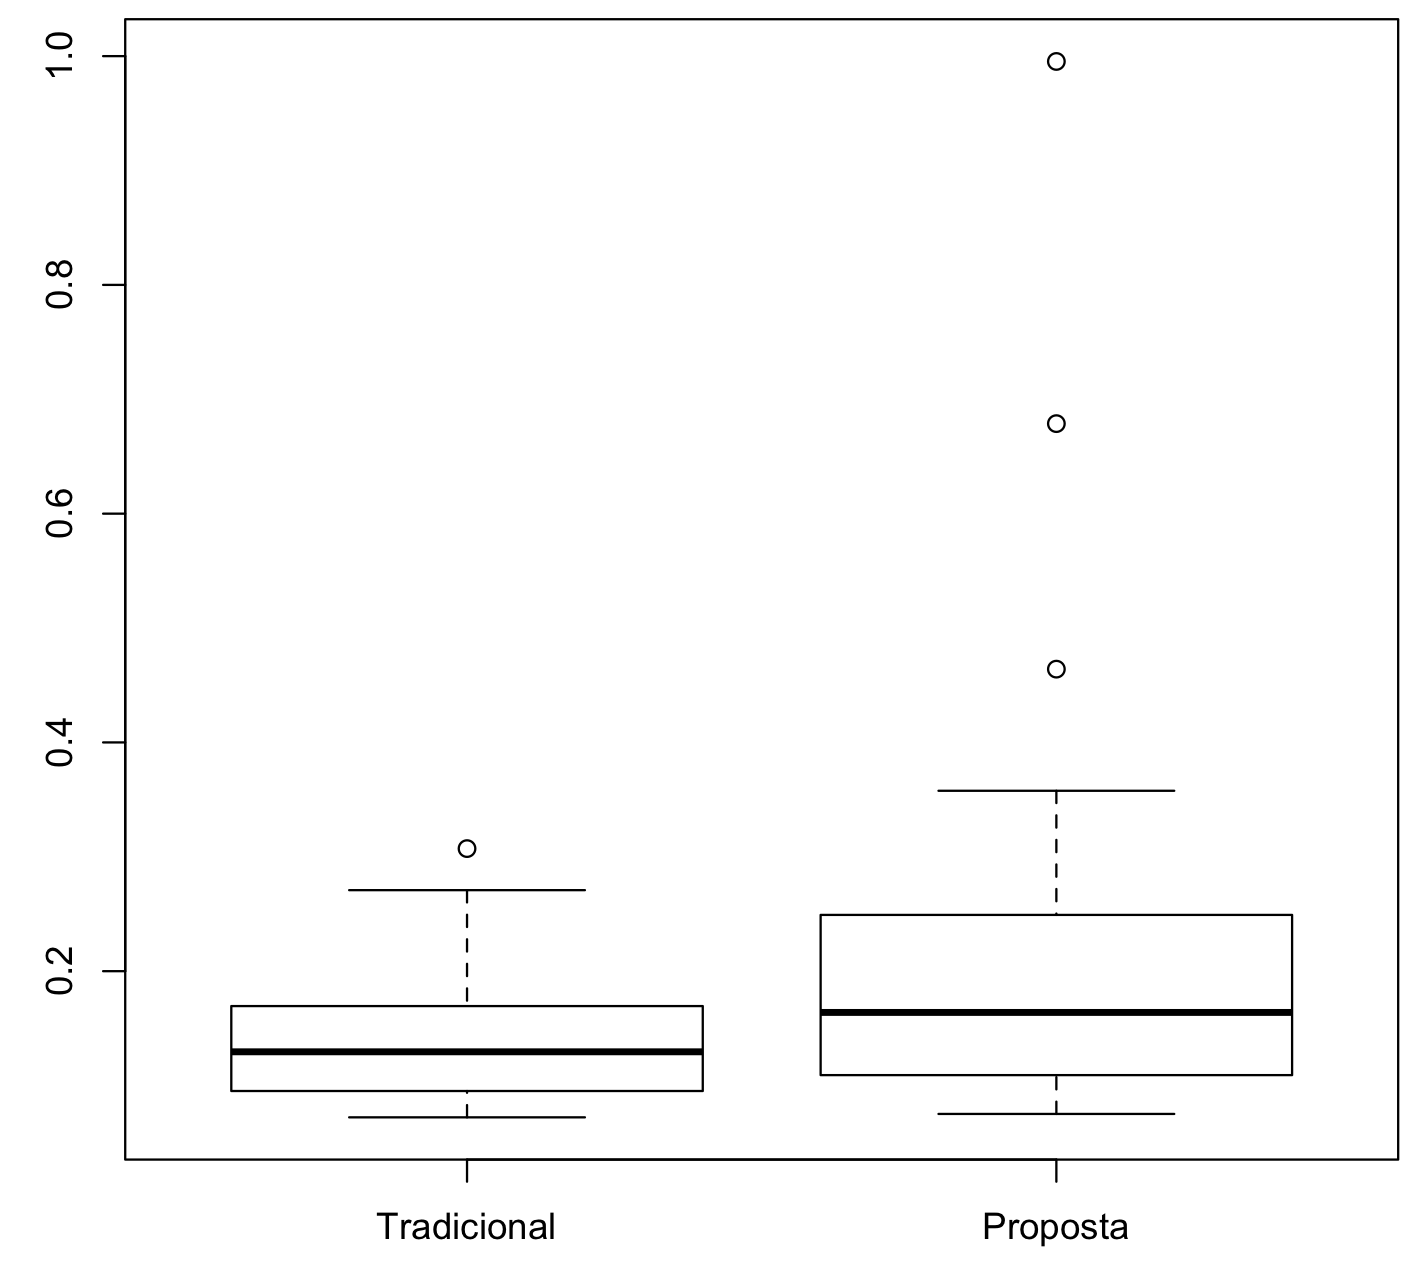
\includegraphics[scale=0.4]{./Figuras/media-harmonica-boxplot.png}
  \end{center}
  \legend{Fonte: O autor.}
\end{figure}

Total de alunos comparados: 85

\begin{multicols}{2}

\noindent\textbf{Tradicional}\\
Min.   :0.07221\\
1st Qu.:0.09545\\
Median :0.12952\\
Mean   :0.13852\\
3rd Qu.:0.16618\\
Max.   :0.30717\\

\columnbreak

\noindent\textbf{Proposta}\\
Min.   :0.07519\\
1st Qu.:0.10913\\
Median :0.16393\\
Mean   :0.21719\\
3rd Qu.:0.24919\\
Max.   :0.99535
\end{multicols}

Shapiro-Wilk normality test

\noindent
data:  data[["media\_harmonica"]]\\
W = 0.63292, p-value = 2.931e-13

\textbf{Resultado: Aceita a hipótese alternativa - Distribuição não normal}

Wilcoxon rank sum test with continuity correction

\noindent
data:  data[["media\_harmonica"]] by data[["algoritmo\_recomendacao"]]\\
W = 634.5, p-value = 0.02082\\
alternative hypothesis: true location shift is not equal to 0

\textbf{Resultado: Aceita a hipótese alternativa - Com diferença significativa}
